\documentclass[aspectratio=169,11pt]{beamer}

\usetheme{Madrid}
\usecolortheme{default}
\usefonttheme{professionalfonts}

\usepackage{graphicx}
\usepackage{booktabs}
\usepackage{array}
\usepackage{hyperref}

\definecolor{ruetblue}{RGB}{15,42,85}
\definecolor{globalblue}{RGB}{37,99,235}
\definecolor{otsuorange}{RGB}{249,115,22}
\definecolor{adaptivegreen}{RGB}{22,163,74}

\setbeamercolor{structure}{fg=ruetblue}
\setbeamercolor{frametitle}{fg=white,bg=ruetblue}
\setbeamercolor{title}{fg=white,bg=ruetblue}
\setbeamertemplate{navigation symbols}{}
\setbeamertemplate{footline}[frame number]

\graphicspath{{../}{assets/}}

\title[Retinal Vessel Segmentation]{Classical Retinal Vessel Segmentation on the FIVES Dataset}
\subtitle{Global, Otsu, and Adaptive Thresholding with Morphology and Skeleton-Based Feature Analysis}
\author[Group 05]{MD. Wariul Mohaimin (2103001) \and Sadman Sakib (2103009)}
\institute[RUET]{Department of Computer Science \& Engineering\\Rajshahi University of Engineering \& Technology}
\date{CSE 4106 -- Digital Image Processing Sessional}

\begin{document}

\begin{frame}
  \titlepage
\end{frame}

\begin{frame}{Presentation Roadmap}
  \begin{columns}[T]
    \begin{column}{0.48\textwidth}
      \begin{enumerate}
        \item Problem and motivation
        \item Dataset and ground truth
        \item Full pipeline architecture
        \item Methodology
        \item Evaluation metrics
      \end{enumerate}
    \end{column}
    \begin{column}{0.48\textwidth}
      \begin{enumerate}
        \setcounter{enumi}{5}
        \item Experimental results
        \item Skeleton and feature analysis
        \item Visual comparison
        \item Final decision
        \item Conclusion
      \end{enumerate}
    \end{column}
  \end{columns}
\end{frame}

\begin{frame}{Problem Motivation}
  \begin{itemize}
    \item Retinal blood vessels are important structures in fundus images.
    \item Manual vessel tracing is slow and subjective.
    \item Vessel segmentation helps measure vessel density, length, width, and fragmentation.
    \item The project uses classical Digital Image Processing methods, so every step is explainable.
  \end{itemize}
  \vspace{0.3cm}
  \begin{block}{Main Question}
    Which classical thresholding method gives the best balance of segmentation quality, feature accuracy, skeleton quality, and speed?
  \end{block}
\end{frame}

\begin{frame}{Dataset}
  \begin{columns}[T]
    \begin{column}{0.52\textwidth}
      \begin{itemize}
        \item Dataset: FIVES retinal vessel dataset.
        \item Evaluation split: 200 test images.
        \item Each image has a manually annotated vessel mask.
        \item Metrics are calculated inside the field-of-view region.
      \end{itemize}
      \vspace{0.2cm}
      \begin{block}{Input and Target}
        Input: color fundus image\\
        Target: binary vessel mask
      \end{block}
    \end{column}
    \begin{column}{0.44\textwidth}
      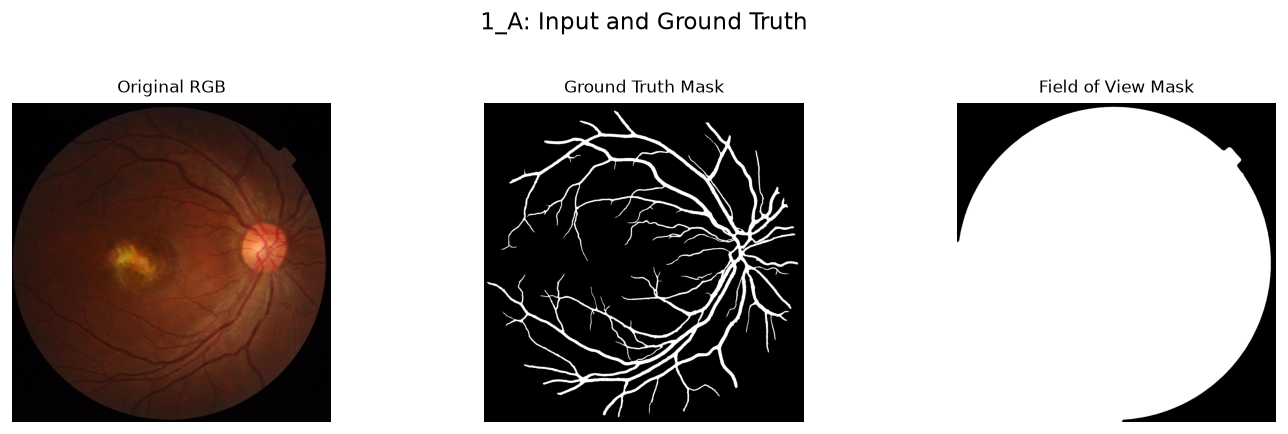
\includegraphics[width=\textwidth]{../notebooks/notebook_outputs/001_1_A_Input_and_Ground_Truth.png}
    \end{column}
  \end{columns}
\end{frame}

{
\usebackgroundtemplate{%
  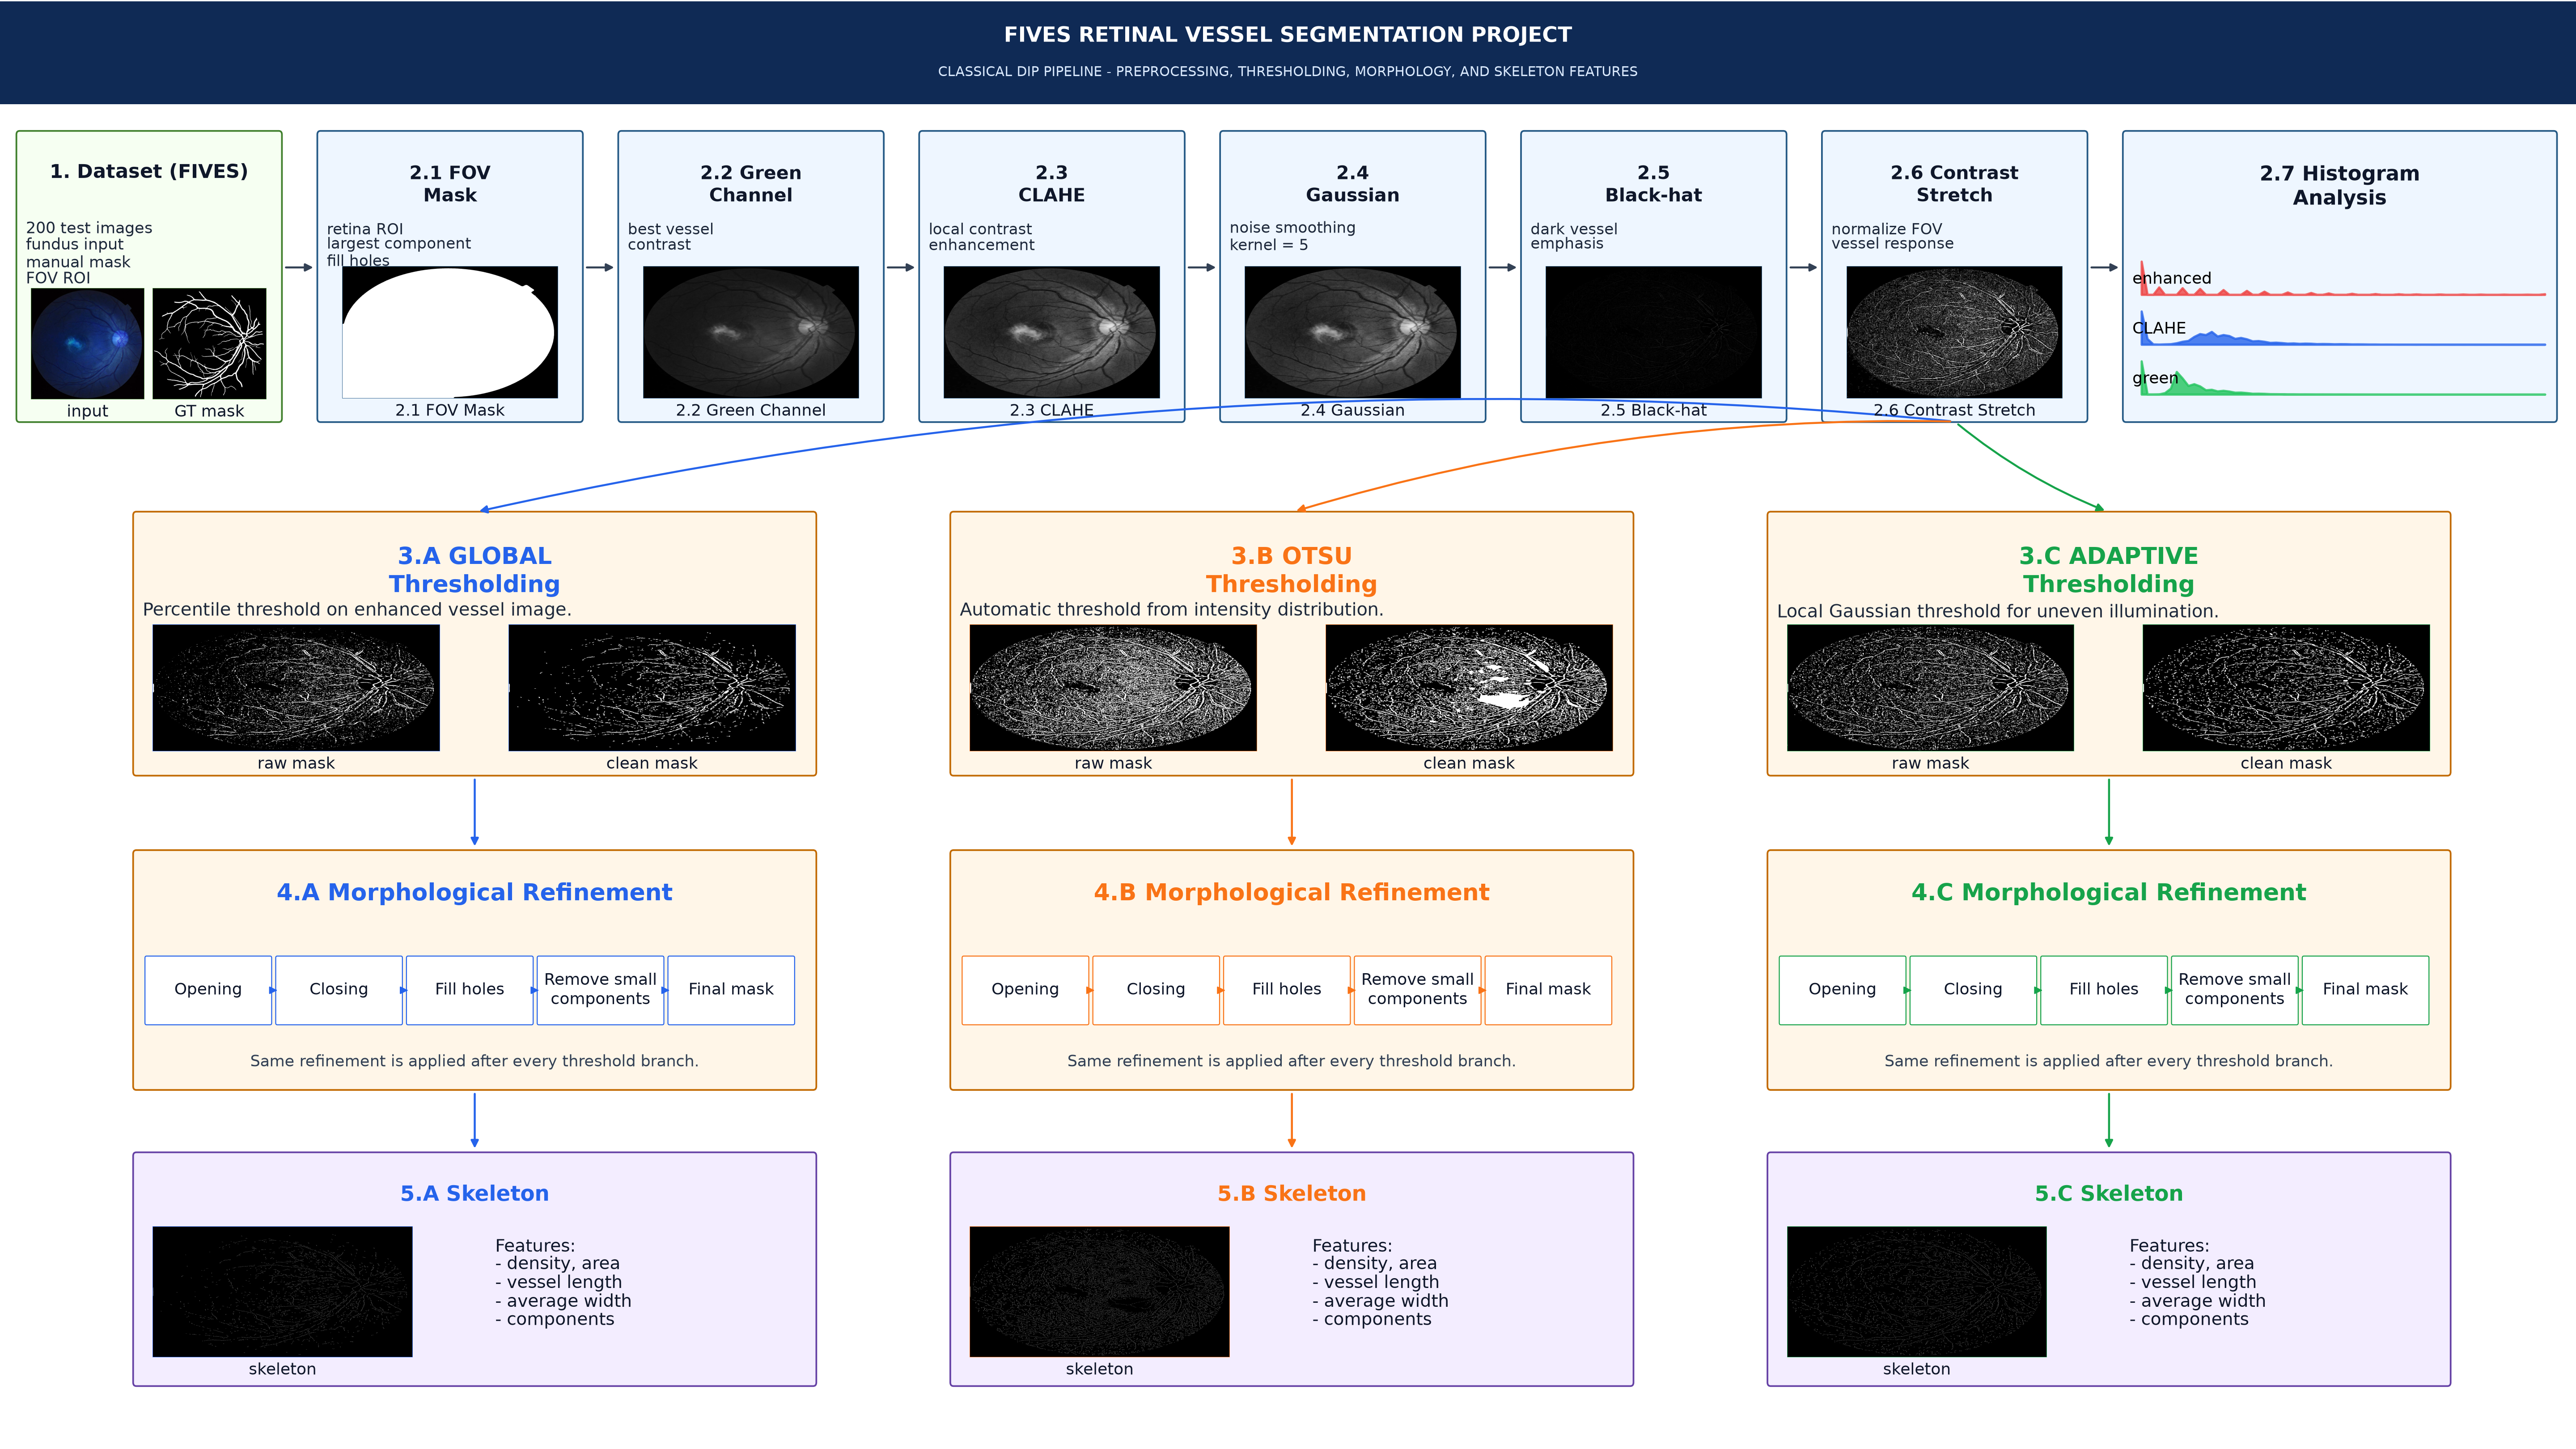
\includegraphics[width=\paperwidth,height=\paperheight]{assets/full_pipeline_architecture.png}%
}
\begin{frame}[plain]
\end{frame}
}

\begin{frame}{Methodology: Preprocessing}
  \begin{columns}[T]
    \begin{column}{0.50\textwidth}
      \begin{enumerate}
        \item Field-of-view detection
        \item Green channel extraction
        \item CLAHE contrast enhancement
        \item Gaussian smoothing
        \item Black-hat morphology
        \item Contrast stretching
      \end{enumerate}
      \vspace{0.2cm}
      \begin{block}{Why Green Channel?}
        Retinal vessels usually appear with stronger contrast in the green channel.
      \end{block}
    \end{column}
    \begin{column}{0.47\textwidth}
      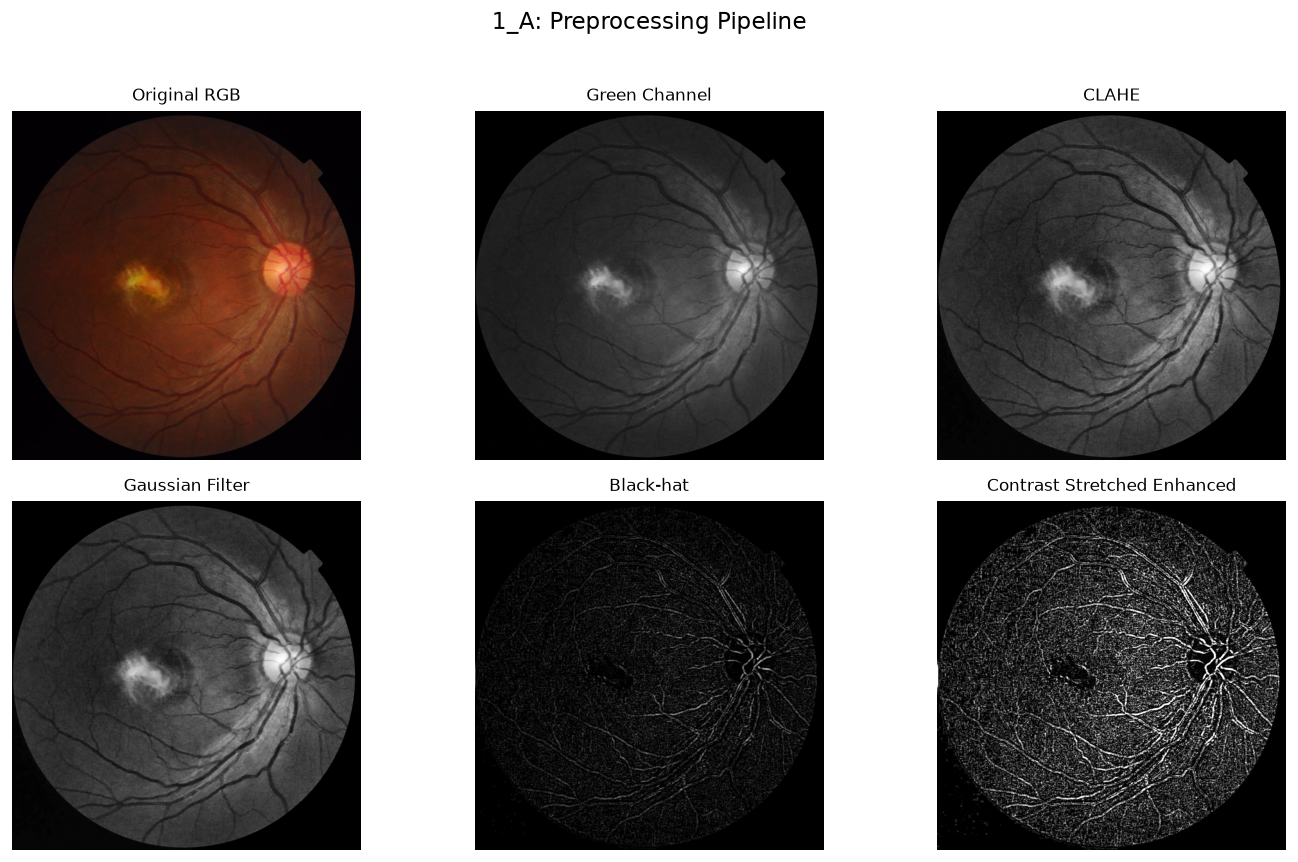
\includegraphics[width=\textwidth]{../notebooks/notebook_outputs/002_1_A_Preprocessing_Pipeline.png}
    \end{column}
  \end{columns}
\end{frame}

\begin{frame}{Segmentation Branches}
  \begin{columns}[T]
    \begin{column}{0.32\textwidth}
      \begin{block}{\textcolor{globalblue}{Global}}
        Percentile threshold on enhanced vessel response. Conservative, usually fewer false positives.
      \end{block}
    \end{column}
    \begin{column}{0.32\textwidth}
      \begin{block}{\textcolor{otsuorange}{Otsu}}
        Automatic threshold using intensity distribution. High recall, but more over-segmentation.
      \end{block}
    \end{column}
    \begin{column}{0.32\textwidth}
      \begin{block}{\textcolor{adaptivegreen}{Adaptive}}
        Local Gaussian thresholding. Handles illumination variation, but can create noisy fragments.
      \end{block}
    \end{column}
  \end{columns}
  \vspace{0.25cm}
  \centering
  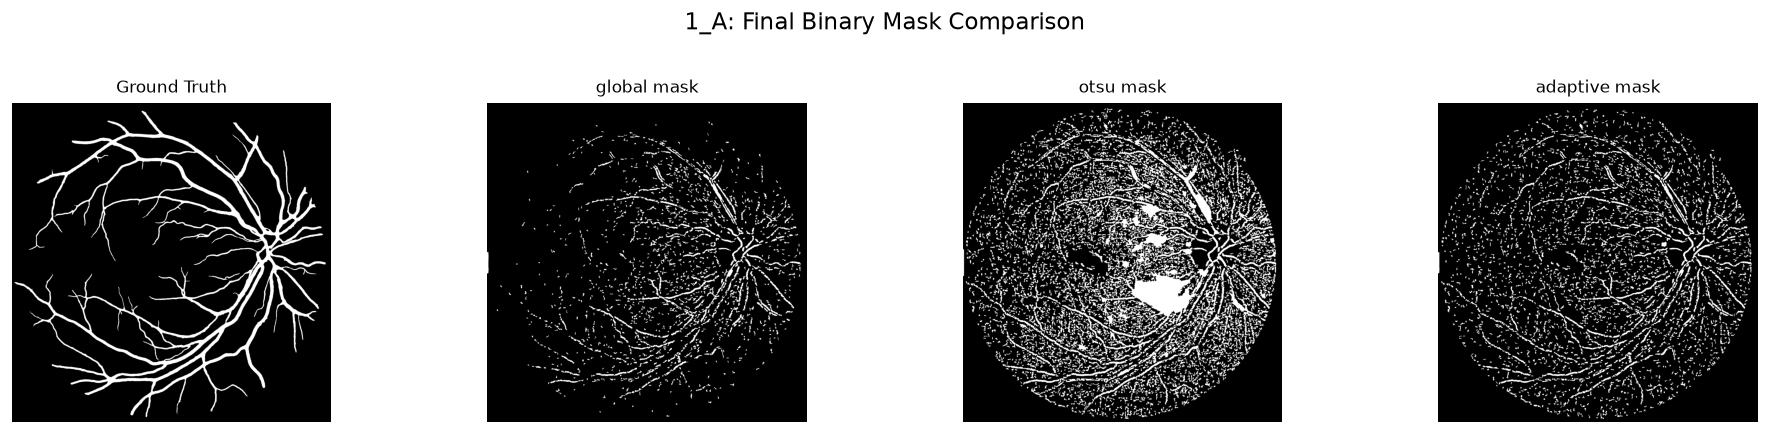
\includegraphics[width=0.88\textwidth,height=0.37\textheight,keepaspectratio]{../notebooks/notebook_outputs/006_1_A_Final_Binary_Mask_Comparison.png}
\end{frame}

\begin{frame}{Morphology and Skeletonization}
  \begin{columns}[T]
    \begin{column}{0.48\textwidth}
      \textbf{Morphological refinement}
      \begin{itemize}
        \item Opening removes isolated noise.
        \item Closing reconnects small breaks.
        \item Hole filling completes vessel regions.
        \item Small-component cleanup reduces false positives.
      \end{itemize}
      \vspace{0.2cm}
      \textbf{Skeletonization}
      \begin{itemize}
        \item Converts vessels to one-pixel-wide centerlines.
        \item Used for vessel length and width estimation.
      \end{itemize}
    \end{column}
    \begin{column}{0.48\textwidth}
      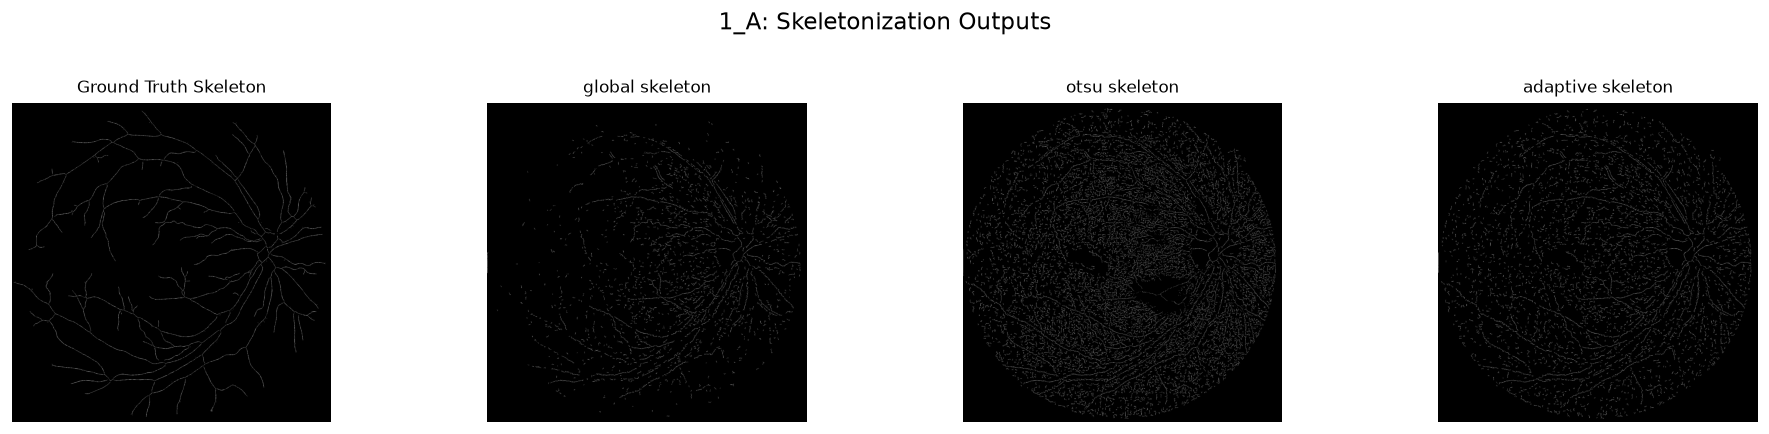
\includegraphics[width=\textwidth]{../notebooks/notebook_outputs/008_1_A_Skeletonization_Outputs.png}
    \end{column}
  \end{columns}
\end{frame}

\begin{frame}{Notebook Pipeline: One Image Step-by-Step}
  \centering
  \begin{columns}[T]
    \begin{column}{0.49\textwidth}
      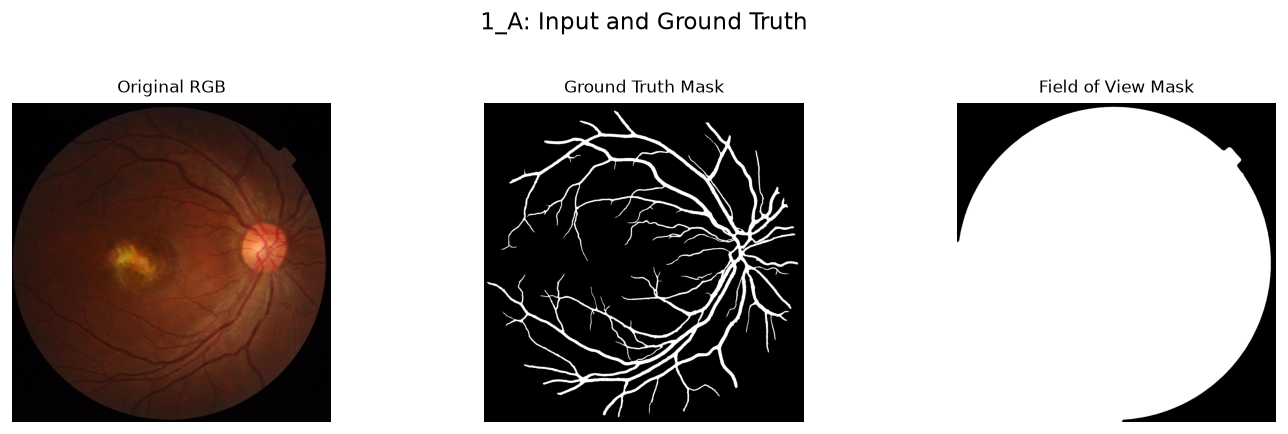
\includegraphics[width=\textwidth,height=0.36\textheight,keepaspectratio]{../notebooks/notebook_outputs/001_1_A_Input_and_Ground_Truth.png}
      \vspace{0.08cm}

      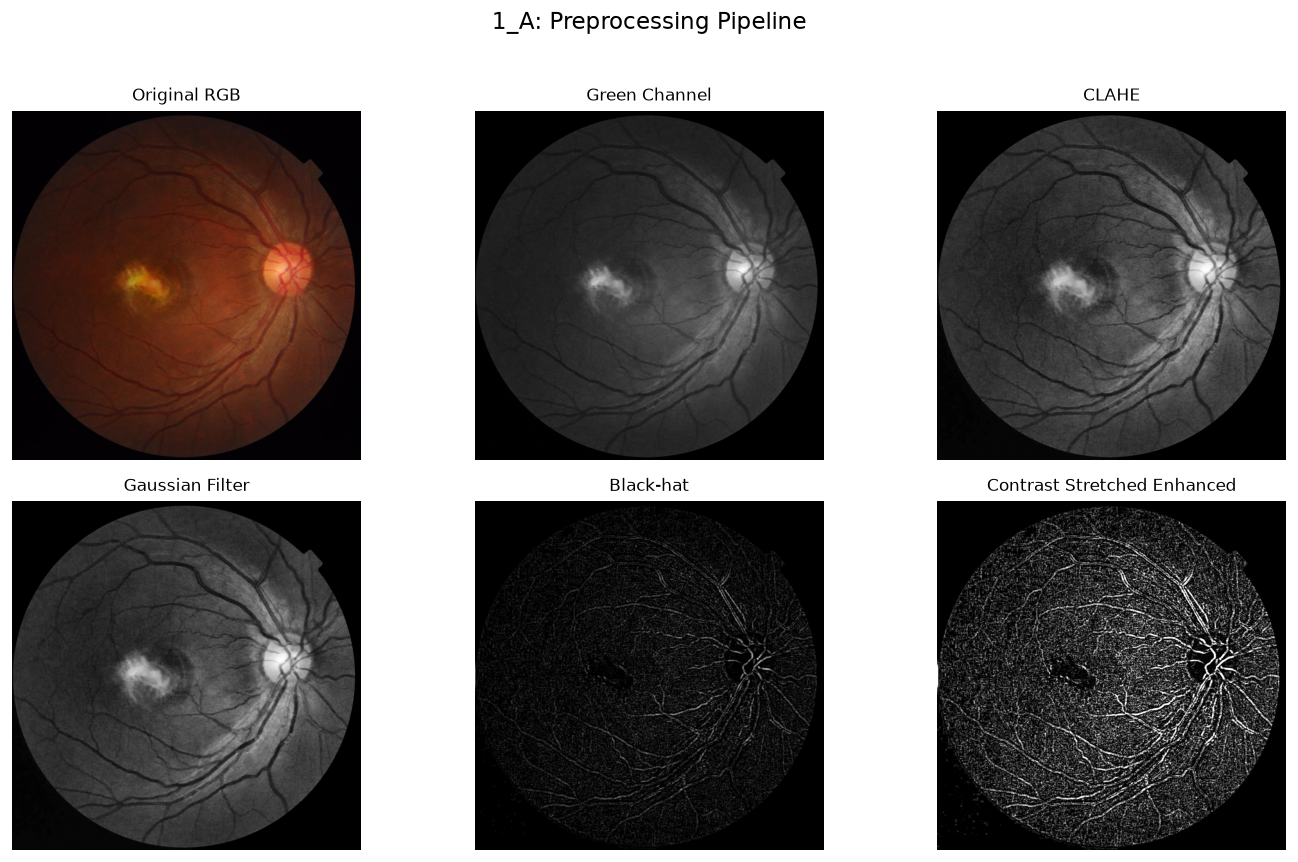
\includegraphics[width=\textwidth,height=0.36\textheight,keepaspectratio]{../notebooks/notebook_outputs/002_1_A_Preprocessing_Pipeline.png}
    \end{column}
    \begin{column}{0.49\textwidth}
      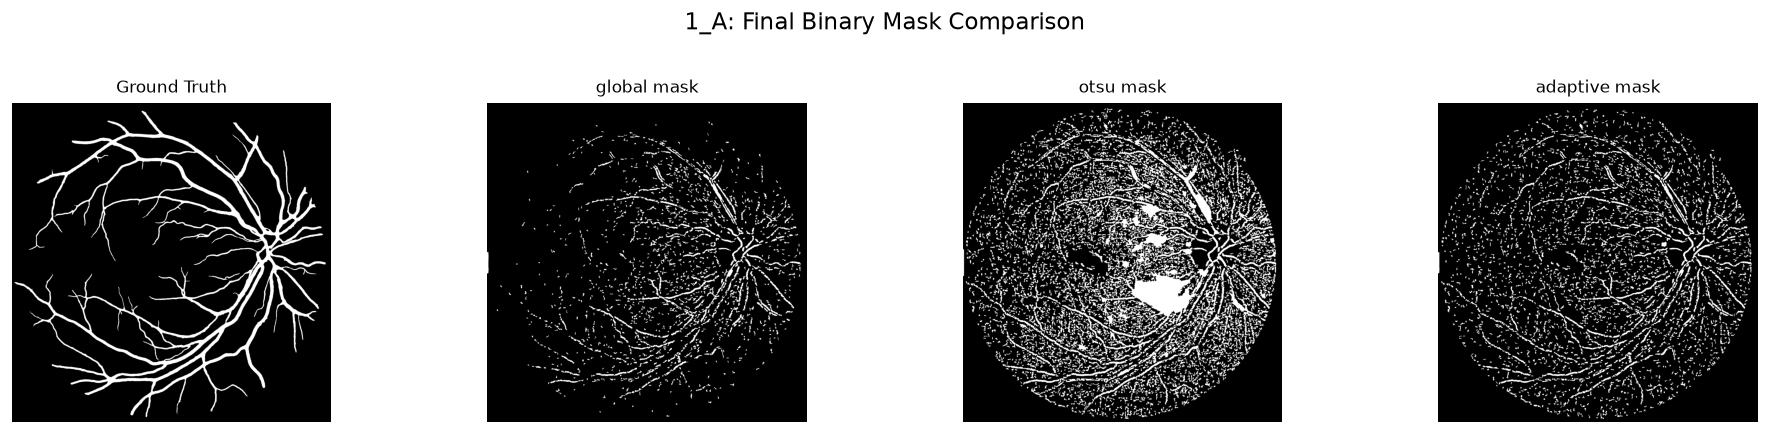
\includegraphics[width=\textwidth,height=0.36\textheight,keepaspectratio]{../notebooks/notebook_outputs/006_1_A_Final_Binary_Mask_Comparison.png}
      \vspace{0.08cm}

      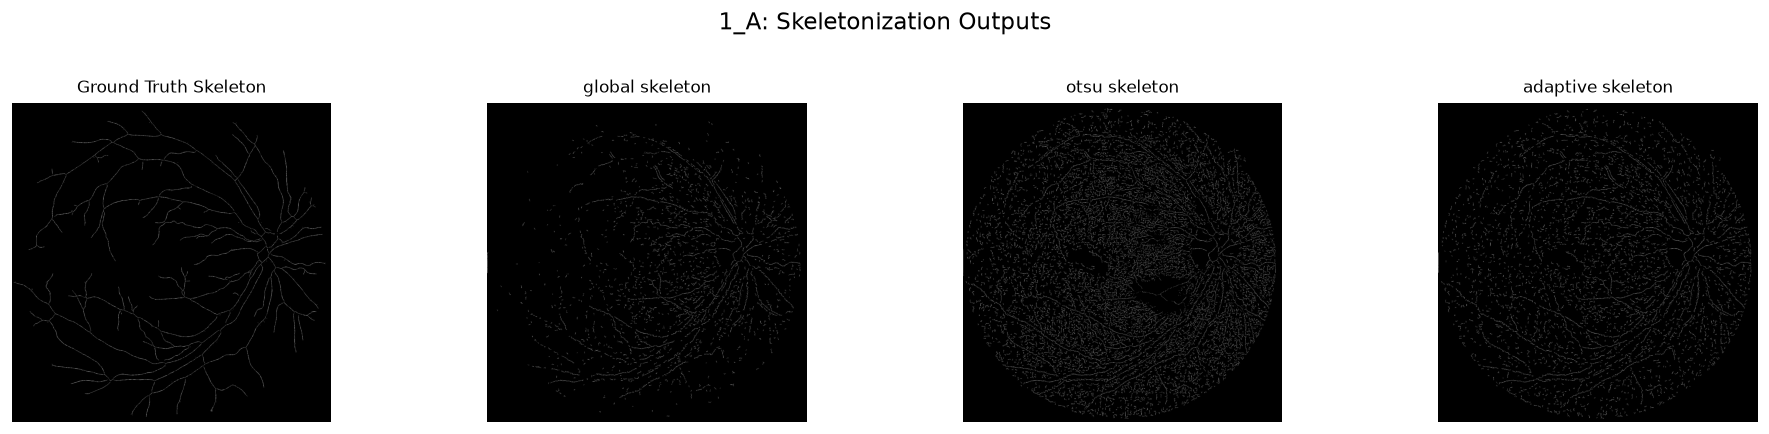
\includegraphics[width=\textwidth,height=0.36\textheight,keepaspectratio]{../notebooks/notebook_outputs/008_1_A_Skeletonization_Outputs.png}
    \end{column}
  \end{columns}
\end{frame}

\begin{frame}{Notebook Pipeline: Threshold Refinement Branches}
  \centering
  \begin{columns}[T]
    \begin{column}{0.33\textwidth}
      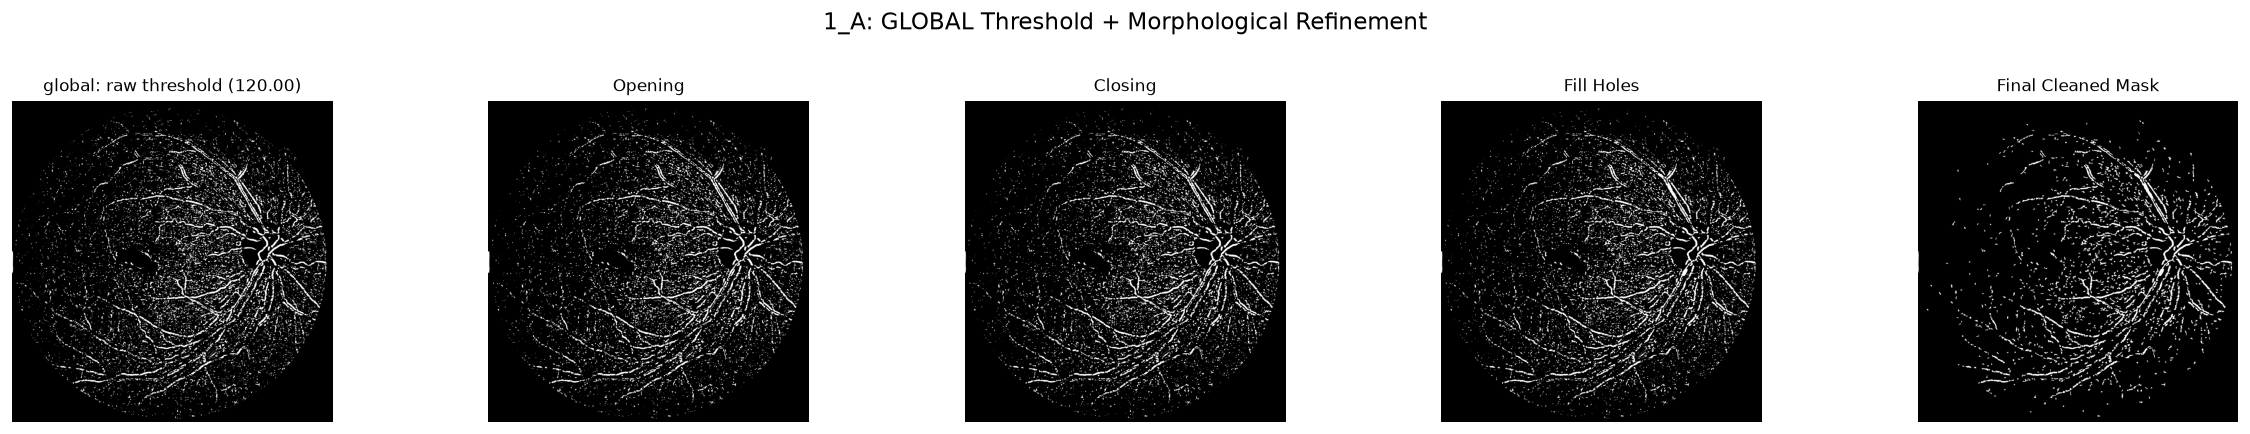
\includegraphics[width=\textwidth,height=0.70\textheight,keepaspectratio]{../notebooks/notebook_outputs/003_1_A_GLOBAL_Threshold_Morphological_Refinement.png}
      \centering\scriptsize Global branch
    \end{column}
    \begin{column}{0.33\textwidth}
      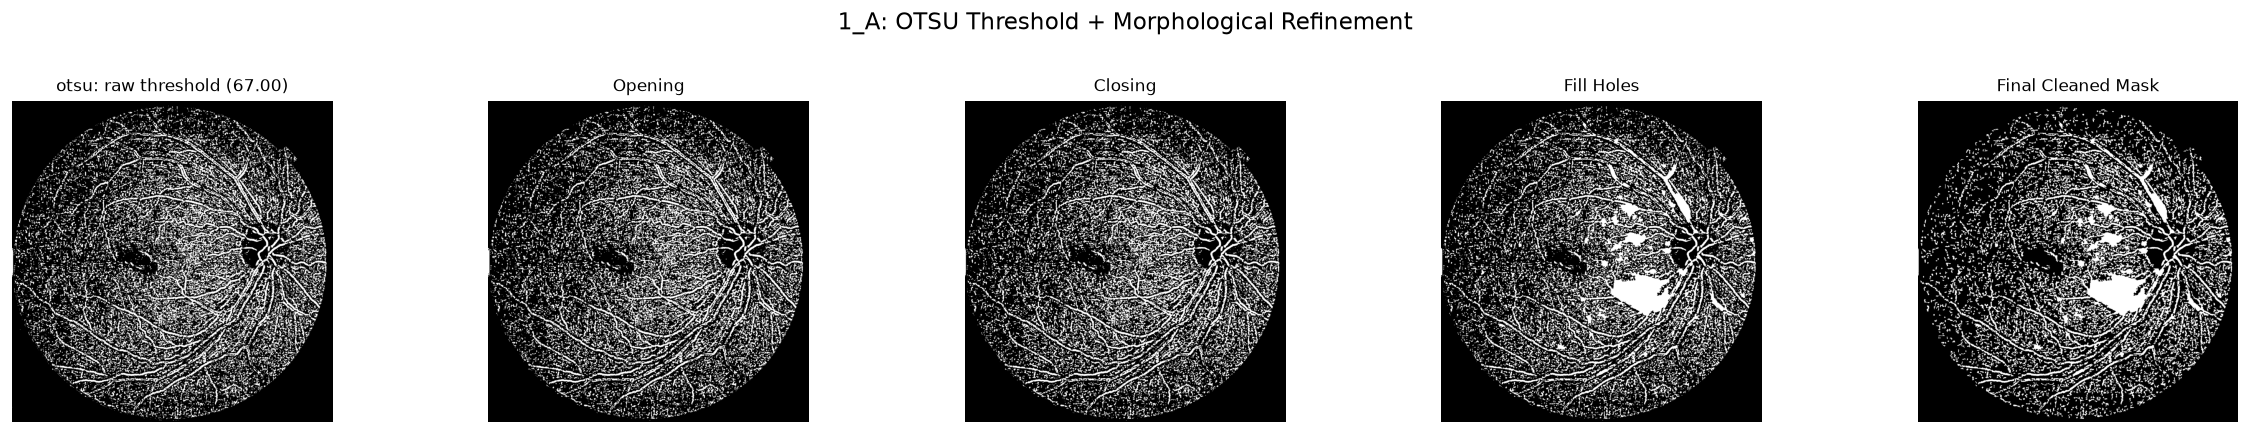
\includegraphics[width=\textwidth,height=0.70\textheight,keepaspectratio]{../notebooks/notebook_outputs/004_1_A_OTSU_Threshold_Morphological_Refinement.png}
      \centering\scriptsize Otsu branch
    \end{column}
    \begin{column}{0.33\textwidth}
      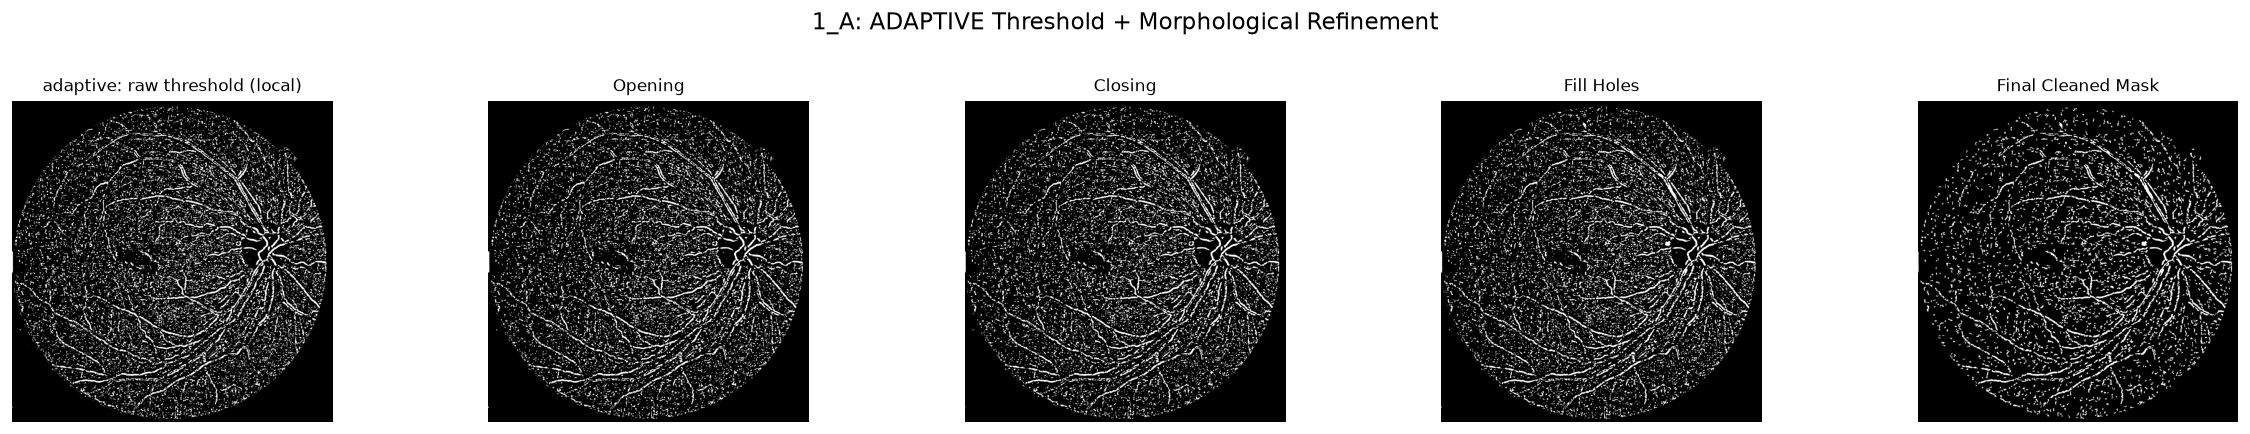
\includegraphics[width=\textwidth,height=0.70\textheight,keepaspectratio]{../notebooks/notebook_outputs/005_1_A_ADAPTIVE_Threshold_Morphological_Refinement.png}
      \centering\scriptsize Adaptive branch
    \end{column}
  \end{columns}
\end{frame}

\begin{frame}{Notebook Pipeline: Overlay Interpretation}
  \begin{columns}[T]
    \begin{column}{0.66\textwidth}
      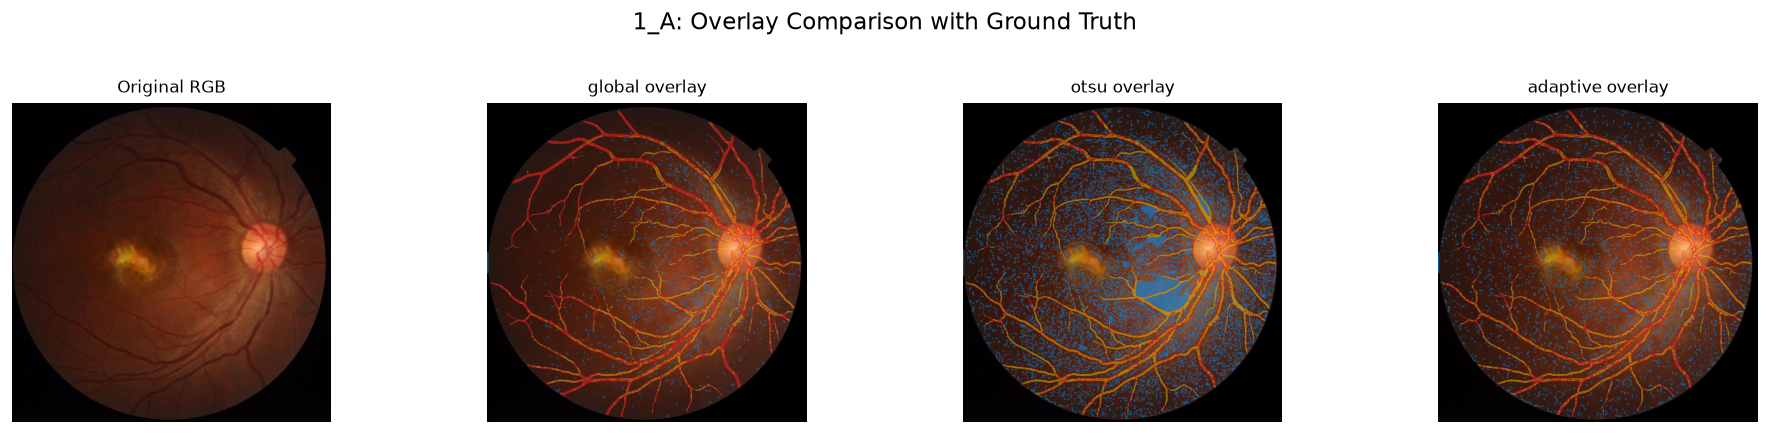
\includegraphics[width=\textwidth,height=0.75\textheight,keepaspectratio]{../notebooks/notebook_outputs/007_1_A_Overlay_Comparison_with_Ground_Truth.png}
    \end{column}
    \begin{column}{0.30\textwidth}
      \begin{block}{Overlay Meaning}
        \scriptsize
        Yellow: true positive vessel pixels\\
        Blue: false positive pixels\\
        Red: missed vessel pixels
      \end{block}
      \scriptsize
      Overlay images are useful because they show \textit{where} the method fails, not only how much it fails.
    \end{column}
  \end{columns}
\end{frame}

\begin{frame}{Evaluation Metrics and Features}
  \begin{columns}[T]
    \begin{column}{0.48\textwidth}
      \textbf{Segmentation metrics}
      \begin{itemize}
        \item Dice, IoU
        \item Precision, Recall, F1
        \item Accuracy
        \item TP, FP, FN, TN pixel counts
      \end{itemize}
    \end{column}
    \begin{column}{0.48\textwidth}
      \textbf{Vessel features}
      \begin{itemize}
        \item Vessel density
        \item Vessel area
        \item Vessel length from skeleton
        \item Average width from distance transform
        \item Connected components
      \end{itemize}
    \end{column}
  \end{columns}
\end{frame}

\begin{frame}{All 200 Images: Metrics Matrix}
  \centering
  \scriptsize
  \begin{tabular}{lrrrrrrrr}
    \toprule
    Method & Images & Dice & IoU & Precision & Recall & F1 & Accuracy & Time(s)\\
    \midrule
    Global & 200 & 0.3819 & 0.2440 & 0.5136 & 0.3135 & 0.3819 & 0.9125 & 0.2713\\
    Otsu & 200 & 0.3041 & 0.1855 & 0.2115 & 0.6742 & 0.3041 & 0.6867 & 1.1929\\
    Adaptive & 200 & 0.3814 & 0.2434 & 0.3411 & 0.4639 & 0.3814 & 0.8629 & 0.3336\\
    \bottomrule
  \end{tabular}
  \vspace{0.35cm}

  \begin{columns}[T]
    \begin{column}{0.47\textwidth}
      \begin{block}{Reading the Matrix}
        \scriptsize
        Each value is the average over all 200 test images. Higher Dice, IoU, precision, recall, F1, and accuracy are better. Lower processing time is better.
      \end{block}
    \end{column}
    \begin{column}{0.47\textwidth}
      \begin{block}{Main Pattern}
        \scriptsize
        Global has the best overall balance. Otsu has the highest recall but also the most false positives. Adaptive is close to Global on Dice/F1 but more fragmented.
      \end{block}
    \end{column}
  \end{columns}
\end{frame}

\begin{frame}{All 200 Images: Feature Error Matrix}
  \centering
  \scriptsize
  \begin{tabular}{lrrrr}
    \toprule
    Method & Density Error & Length Error & Width Error & Component Error\\
    \midrule
    Global & 3.8673 & 8586.75 & 7.2765 & 1144.77\\
    Otsu & 25.4285 & 111918.63 & 5.9090 & 2179.27\\
    Adaptive & 4.5758 & 56381.28 & 7.4194 & 2643.67\\
    \bottomrule
  \end{tabular}
  \vspace{0.25cm}

  \includegraphics[width=0.78\textwidth,height=0.46\textheight,keepaspectratio]{../results_test/visual_report/charts/test_feature_error_heatmap.png}
\end{frame}

\begin{frame}{Average Segmentation Results}
  \centering
  \begin{tabular}{lrrrrrr}
    \toprule
    Method & Dice & IoU & Precision & Recall & F1 & Accuracy\\
    \midrule
    Global & 0.3819 & 0.2440 & 0.5136 & 0.3135 & 0.3819 & 0.9125\\
    Otsu & 0.3041 & 0.1855 & 0.2115 & 0.6742 & 0.3041 & 0.6867\\
    Adaptive & 0.3814 & 0.2434 & 0.3411 & 0.4639 & 0.3814 & 0.8629\\
    \bottomrule
  \end{tabular}
  \vspace{0.35cm}
  \includegraphics[width=0.86\textwidth,height=0.43\textheight,keepaspectratio]{../results_test/visual_report/charts/test_segmentation_metric_comparison.png}
\end{frame}

\begin{frame}{All 200 Images: Best Method by Criterion}
  \centering
  \scriptsize
  \begin{tabular}{llr}
    \toprule
    Criterion & Best Method & Value\\
    \midrule
    Highest Dice & Global & 0.3819\\
    Highest IoU & Global & 0.2440\\
    Highest Precision & Global & 0.5136\\
    Highest Recall & Otsu & 0.6742\\
    Highest F1 & Global & 0.3819\\
    Highest Accuracy & Global & 0.9125\\
    Fastest Processing Time & Global & 0.2713\\
    Lowest Density Error & Global & 3.8673\\
    Lowest Length Error & Global & 8586.75\\
    Lowest Width Error & Otsu & 5.9090\\
    \bottomrule
  \end{tabular}
  \vspace{0.25cm}

  \begin{block}{Interpretation}
    Global wins most criteria. Otsu wins recall and width error, but its over-segmentation makes its overall rank worse.
  \end{block}
\end{frame}

\begin{frame}{Feature Error Analysis}
  \begin{columns}[T]
    \begin{column}{0.50\textwidth}
      \includegraphics[width=\textwidth]{../results_test/visual_report/charts/test_feature_error_heatmap.png}
    \end{column}
    \begin{column}{0.46\textwidth}
      \begin{itemize}
        \item Global has the lowest density error.
        \item Global has the lowest vessel length error.
        \item Otsu has the lowest average width error.
        \item Otsu over-segments, increasing predicted area and skeleton pixels.
      \end{itemize}
    \end{column}
  \end{columns}
\end{frame}

\begin{frame}{Feature Values: Prediction vs Ground Truth}
  \centering
  \includegraphics[width=\textwidth,height=0.78\textheight,keepaspectratio]{../results_test/visual_report/charts/test_feature_values_predicted_vs_ground_truth.png}
\end{frame}

\begin{frame}{Confusion Pixel Summary}
  \begin{columns}[T]
    \begin{column}{0.58\textwidth}
      \includegraphics[width=\textwidth,height=0.70\textheight,keepaspectratio]{../results_test/visual_report/charts/test_confusion_pixel_summary.png}
    \end{column}
    \begin{column}{0.38\textwidth}
      \begin{itemize}
        \item TP: correctly detected vessel pixels.
        \item FP: predicted vessel but actually background.
        \item FN: missed vessel pixels.
        \item Otsu increases recall by predicting more vessel pixels, but that also increases FP.
      \end{itemize}
    \end{column}
  \end{columns}
\end{frame}

\begin{frame}{Skeleton Branch Results}
  \begin{columns}[T]
    \begin{column}{0.50\textwidth}
      \includegraphics[width=\textwidth]{../results_test/visual_report/charts/test_skeleton_metric_comparison.png}
    \end{column}
    \begin{column}{0.46\textwidth}
      \begin{itemize}
        \item Skeleton metrics compare predicted centerlines with ground-truth centerlines.
        \item Global skeleton is more conservative.
        \item Otsu predicts many more skeleton pixels, increasing recall but lowering precision.
        \item Skeletonization is necessary for length and width calculations.
      \end{itemize}
    \end{column}
  \end{columns}
\end{frame}

\begin{frame}{Representative Cases from Notebook}
  \centering
  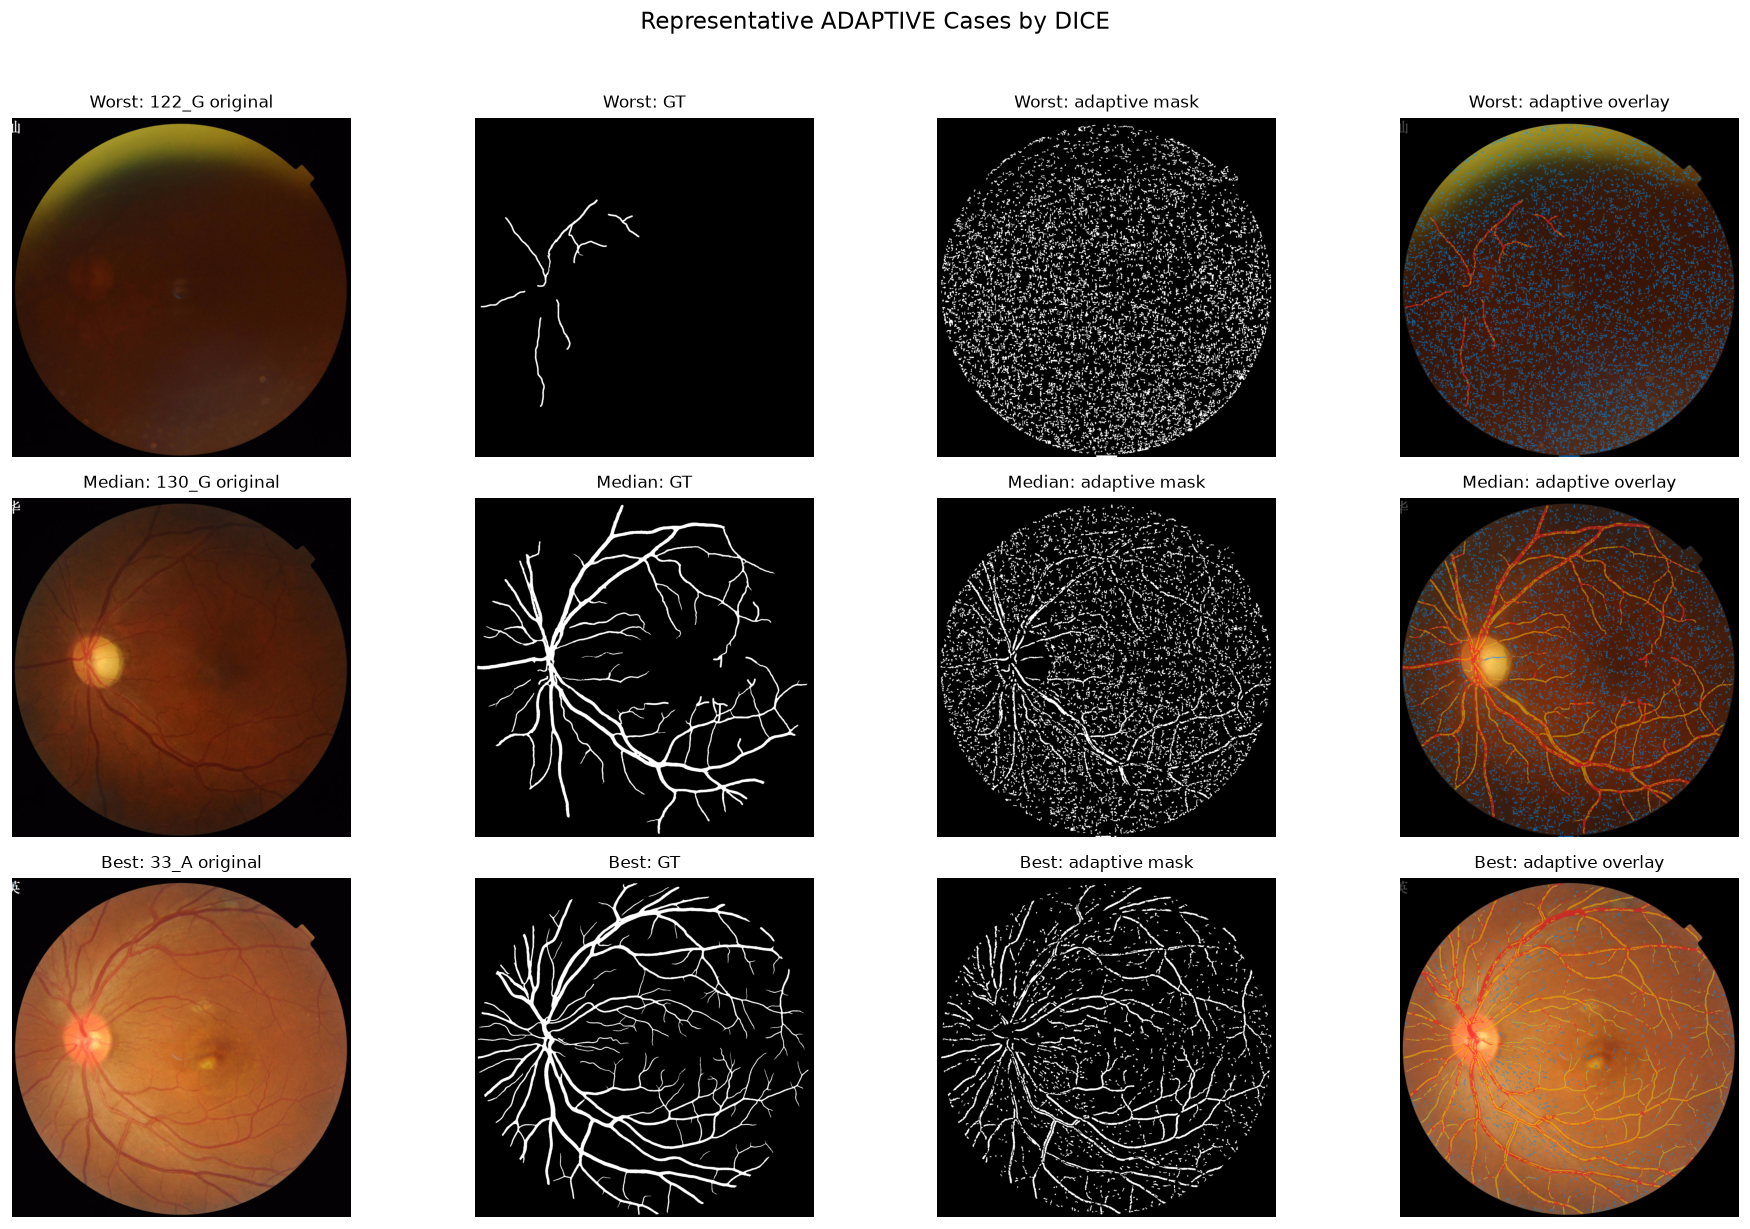
\includegraphics[width=\textwidth,height=0.78\textheight,keepaspectratio]{../notebooks/notebook_outputs/034_Representative_ADAPTIVE_Cases_by_DICE.png}
\end{frame}

\begin{frame}{Processing Time and Overall Ranking}
  \begin{columns}[T]
    \begin{column}{0.50\textwidth}
      \includegraphics[width=\textwidth]{../results_test/visual_report/charts/test_processing_time.png}
    \end{column}
    \begin{column}{0.46\textwidth}
      \includegraphics[width=\textwidth]{../results_test/visual_report/charts/test_overall_method_ranking.png}
      \vspace{0.2cm}
      \begin{block}{Final Ranking}
        1. Global\\
        2. Adaptive\\
        3. Otsu
      \end{block}
    \end{column}
  \end{columns}
\end{frame}

\begin{frame}{Visual Comparison}
  \centering
  \includegraphics[width=\textwidth,height=0.78\textheight,keepaspectratio]{../results_test/figures/test_1_A_comparison.png}
  \vspace{0.1cm}

  \footnotesize Overlay colors: yellow = true positive, blue = false positive, red = false negative.
\end{frame}

\begin{frame}{Key Findings}
  \begin{enumerate}
    \item Global thresholding is the best overall method on the test set.
    \item Otsu gives the highest recall but creates many false positives.
    \item Adaptive thresholding is competitive but more fragmented.
    \item Skeletonization is essential for vessel length and width estimation.
    \item Accuracy alone is not enough because background pixels dominate retinal images.
  \end{enumerate}
\end{frame}

\begin{frame}{Conclusion}
  \begin{block}{Final Decision}
    Global thresholding gives the strongest balance of overlap score, feature error, processing time, and visual quality.
  \end{block}
  \begin{itemize}
    \item The final pipeline uses green-channel enhancement, three thresholding branches, morphology, and skeleton analysis.
    \item Edge detection and watershed were removed to keep the project focused and explainable.
    \item The project produced masks, skeletons, overlays, CSV tables, dashboard charts, notebook figures, and a LaTeX report.
  \end{itemize}
\end{frame}

\begin{frame}{Future Work}
  \begin{itemize}
    \item Tune threshold and morphology parameters per method.
    \item Add vessel-specific enhancement filters such as Frangi filtering.
    \item Detect branch points and endpoints from skeletons.
    \item Compare the classical pipeline with a deep learning model.
    \item Evaluate more splits or external retinal datasets.
  \end{itemize}
  \vspace{0.4cm}
  \centering
  \Large Thank You
\end{frame}

\end{document}
